\chapter*{JavaScriptSchema}\stepcounter{chapter}
\addcontentsline{toc}{chapter}{JavaScriptSchema}
%\chapter{JavaScriptSchema átírása}\label{chap:JavaScriptSchema átírása}
\section{A JavaScriptSchemáról}

\noindent

A JavaScriptSchéma egy UML Diagramhoz hasonlító schéma. Jelen esetben a Visual Paradigm alkalmazással szerkeszthető.
A felépítése a következőképpen alakul:

\begin{figure}[!htbp]
      \caption{JavaScriptSchema struktúrális felépítése}\label{fig:JavaScriptSchema_struktura}
      \centering
      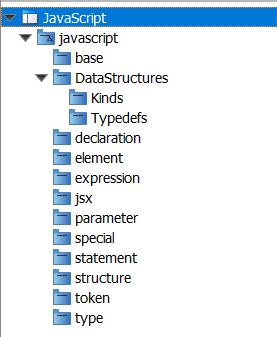
\includegraphics[width=0.4\textwidth]{JavaScriptSchema_struktura.png}
\end{figure}

\Aref{fig:JavaScriptSchema_struktura} ábrán a következő struktúra figyelhető meg: ProjektNév-Model-Packagek.
A projekt neve a JavaScript, ezen belül található egy model, amit javascript-nek hívnak. A modellen belül találhatóak meg a packagek.
A Packagek nem véletlenül így lettek elnevezve. Az alábbi hivatkozáson található meg, hogy milyen logika alapján neveztük el a packageket:~\cite{typescript-eslint}
Nem feltétlenül muszáj több packaget létrehozni, ez csupán az átláthatóság és a könnyen bővíthetőség céljából lett így megvalósítva.
Követtük a typescript-eslint githubon lévő projekt struktúrális logikáját, több helyen is eltértünk tőle, mivel a mi projektünk másabb, illetve speciális megoldásokat igényelt egyes helyeken.
A következő oldalakon bemutatom a packagek felépítését néhány egyszerűbb példán szemléltetve.
A packagek a következőképpen épülnek fel:
\begin{figure}[!htbp]
      \caption{A base package felépítése}\label{fig:base_vpp}
      \centering
      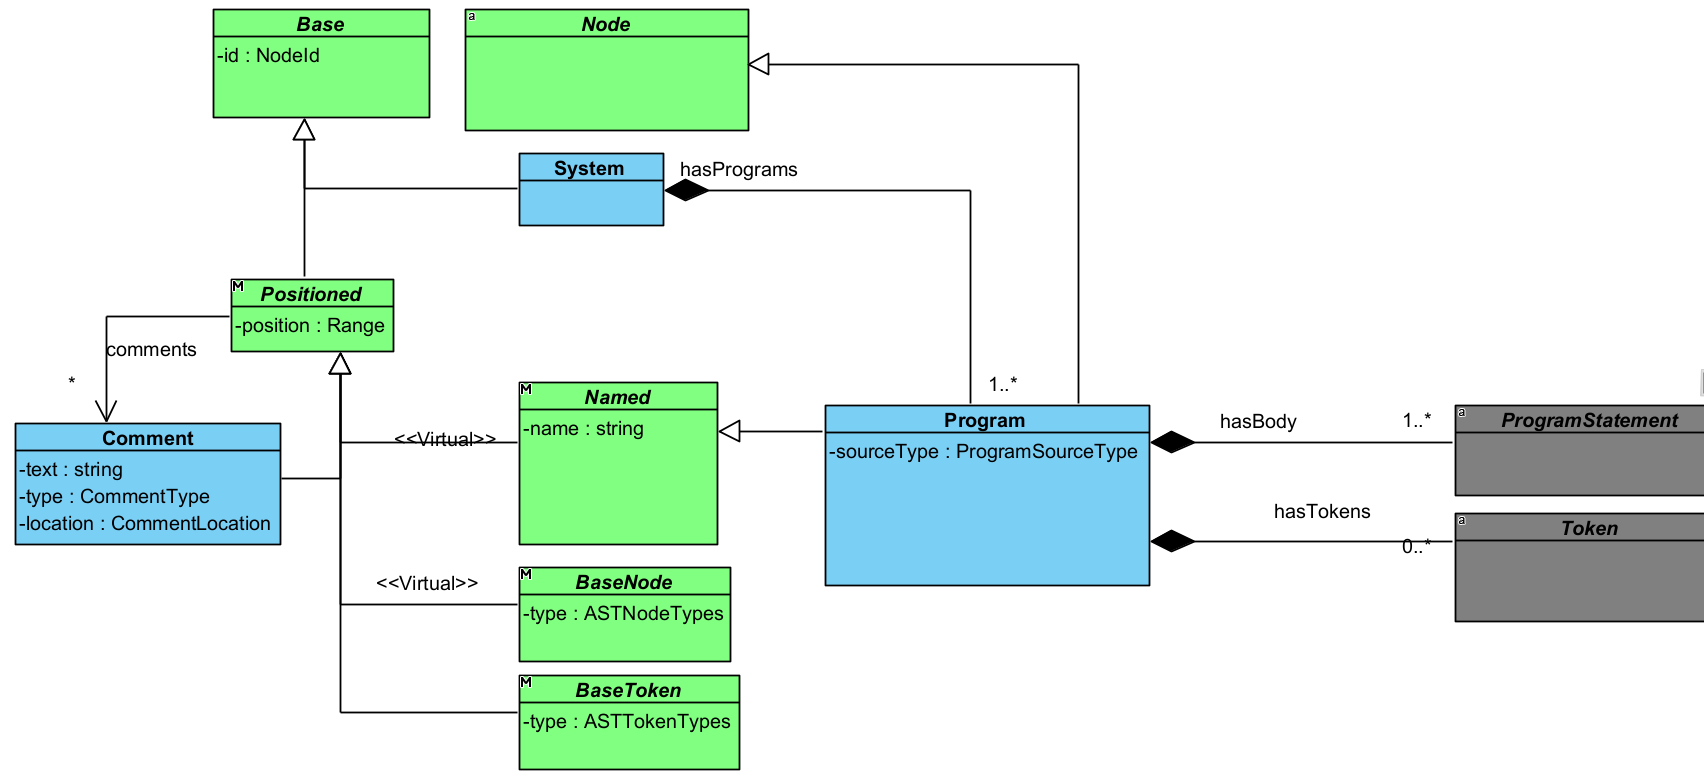
\includegraphics[width=0.9\textwidth]{base_vpp.png}
\end{figure}

\Aref{fig:base_vpp} ábrán különböző osztályok láthatóak. A Base osztály mindennek az alapja, ebből öröklődik minden más.
Látható, hogy egy id attribútummal rendelkezik, aminek a típusa NodeId.
A zöld háttérszínű osztályok az absztrakciót jelentik. Működésben nincs jelentősége, csak a schéma szerkeszthetősége és olvashatósága miatt van így jelezve.
A szürke háttérszínű osztályok pedig csupán annyit jelentenek, hogy más packageben lettek definiálva.
A kék a default, normális osztályt jelölik.
A Positioned és a System származik le a Baseből, értelemszerűen a system az maga a program lesz.
A Positioned az azért absztrakt, mivel majd ebből fognak leszármazni a kisebb osztályok, mint például az expression, statement és a többi.
A Positioned osztálynak van egy attribútuma, a poisition, ami egy Range típus. Emellett még tartozhatnak hozzá kommentek is.
A komment egyaránt leszármazik a positioned-ből, ezzel garantálva azt, hogy a kommentnek van pozíciója.
Látható, hogy a kommentnek van egy text, type és location attribútuma. A CommentType és a CommentLocation a DataStructures-ben van definiálva.
Emellett a Named, BaseNode és a BaseToken származik le a Positionedből. A Named osztály azt jelenti, hogy egy nodenak van-e name attribútuma vagy sem.
A BaseNodeból és a BaseTokenből fog nagyon sok minden leszármazni aminek van typeja.
Végül, megtalálható a Program osztály, aminek van name attribútuma, mivel Named-ből származik le, és van Systeme. Az 1..* jelenti azt, hogy legalább 1 Systeme van, de lehet több is.
A hasPrograms-nak majd máshol lesz jelentősége, a mi esetünkben majd a javascriptben.
Tetszőlegesen el lehet nevezni, de konzisztencia miatt, minden attribútum ami osztály (és nem a DataStructuresben azon belül is a Kindsban van definiálva, hanem van neki egy osztály, mint pl Comment)
azt a hasOsztály névvel fogjuk ellátni.
A ProgramSourceType is a Kinds packageben van definiálva, ami csupán azt mondja meg, hogy az adott program vagy script vagy module típusú.
A base package nem követi a typescript-eslint githubon lévő projekt base mappáját, ez teljesen egyedi, átememeltük az egészet apróbb módosítással az előző projekt verzióból.

\noindent

A base packagen kívül bemutatom a declaration packaget, hogy lássuk milyen logikát követtünk a megírás során.
Ezen belül is az ExportAllDeclaration bemutatása:

\begin{lstlisting}[caption={ExportAllDeclaration typescriptes megvalósítása},label={lst:ExportAllDeclaration}, language={JavaScript}]
export interface ExportAllDeclaration extends BaseNode {
      type: AST_NODE_TYPES.ExportAllDeclaration;
      assertions: ImportAttribute[];
      exported: Identifier | null;
      exportKind: ExportKind;
      source: StringLiteral;
}
\end{lstlisting}

\Aref{lst:ExportAllDeclaration} kódrészlet így lett megvalósítva a JavaScriptSchémában:

\begin{figure}[!htbp]
      \caption{A declaration package felépítése}\label{fig:declaration_vpp}
      \centering
      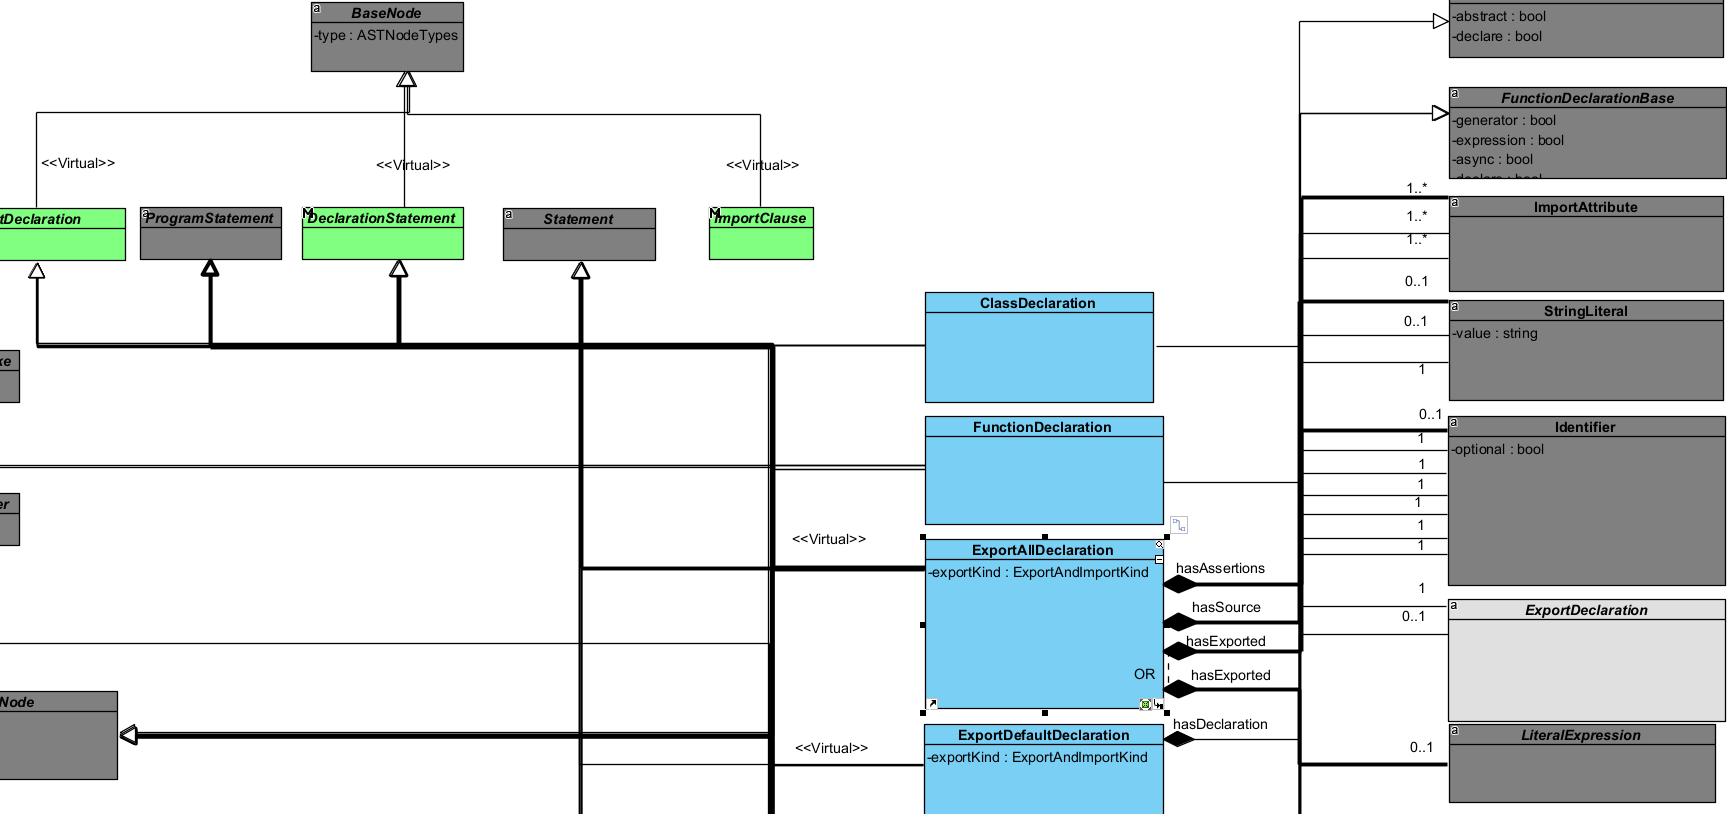
\includegraphics[width=1\textwidth]{declaration.png}
\end{figure}

\Aref{fig:declaration_vpp} ábrán látható az, hogy minden a BaseNodeból származik. \Aref{lst:ExportAllDeclaration} kódrészletben ez az extends BaseNode.
Itt maga a declaration osztály az a DeclarationStatement névre hallgat, csupán azért, mert követtük a typescriptes kódot. A főbb osztályok a BaseNode alatt találhatóak.
Jobb oldalt a sötétszürke és a világosszürke osztályok azok az attribútumok.
Ebben az esetben az ExportAllDeclaration osztály leimplementálását mutatom be a JavaScriptSchemában.
Az ExportAllDeclaration öröklődik a Statement, DeclarationStatement, Node és a ProgramStatementből.
Ezeket az öröklődéseket ugyanúgy a typescript-eslint githubról néztük, unions mappában érhetőek el.
Ezáltal megkapja az összes szülőnek a tulajdonságait. A DeclarationStatement öröklődik a BaseNodeból, ami azt jelenti, hogy a BaseNode tulajdonságait is megkapja az ExportAllDeclaration.
A BaseNode ugye meg származik a Positionedből, ez látható \aref{fig:base_vpp} ábrán.
Emiatt az ExportAllDeclaration-nek lesz pozíciója, kommentje és NodeId-ja is.
Assertions attribútum típusa az ImportAttribute, látható, hogy egy tömböt vár, ezért 1..* a multiplicityje.
Exported attribútumnál egy Identifier típusú attribútumot vár, itt mi kiegészítettük még egy LiteralExpressiönnel is, ami maga a Literal.
A vagyolást egy OR-al jeleztük a JavaScriptSchemában.
Mivel lehet null-is, ezért 0..1 a multiplicity, szóval vagy 0 vagy 1.
Az ExportKind az a Kindsban található meg, így szimplán csak arra hivatkozunk, mint ExportAndImportKind.
Végül a source attribútuma egy StringLiteral, nálunk is így szerepel.
Természetesen ami sötétszürkével van jelölve, az máshol létre van hozva és vannak neki attribútumai.
A világosszürke annyit jelöl, hogy ebben a packageben lett létrehozva az osztály, de láthatóság szempontból többször szerepel, mivel lehet attribútum is.
Így lett minden egyes osztály felépítve, természetesen \Aref{fig:declaration_vpp} ábra csak egy részlete a declaration packagenek, ennél jóval nagyobb.
Vannak úgynevezett gyűjtő osztályok is, mint pl a Statement, ezekre azért van szükség, mert majd később ha le lett generálva minden, akkor tudjunk majd vizsgálni különböző nodeokra, mint például isStatement().

\noindent

Sokat említettem a DataStructurest. Hadd mutassam be egy példán keresztül, hogy ez hogy néz ki:

\begin{figure}[!htbp]
      \caption{A DataStructures packageben a Kind package felépítése}\label{fig:data_structures_kinds}
      \centering
      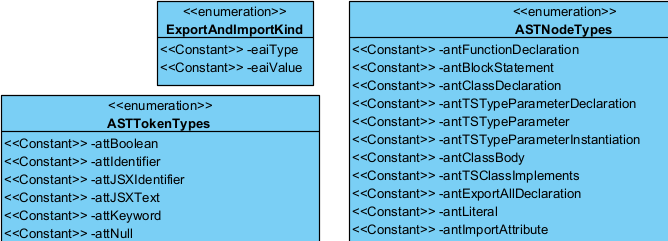
\includegraphics[width=0.6\textwidth]{data_structures.png}
\end{figure}

A DataStructures packageben található 2 package, ez \aref{fig:JavaScriptSchema_struktura} ábrán látható. Ebből a Kinds packaget mutatom be.
\Aref{fig:data_structures_kinds} ábrán látható egy kis szelet a Kinds packageből.
Enumok találhatóak ebben a packageben.
Például ha az ExportAndImportKind-ot adjuk meg típusnak az egyik attribútumnak, akkor az lehet vagy eaiType vagy eaiValue.
Minden constant előtt van 3 karakter, ez azért szükséges, mert később ezekkel még foglalkozni fogunk.

\noindent

A JavaScriptSchema magában még semmit sem csinál. Először ki kell exportálni az egész projectet xml formátumba.
Ezután az xml filet átkonvertáljuk egy asg filera. Ez úgy történik, hogy a JavaScript Analyzer projektnek van egy kisebb alprojektje, amit UmlToAsg-nek hívnak.
Ez a java kód átkonvertálja az xml fileban lévő adatot egy asg fileba. Jobban nem térnék ki az UmlToAsg projektre, mivel nem szerkesztettük.
Az UmlToAsg projektet a SchemaGenerator generálta le. A SchemaGenerator c++ nyelven megírt program. Több mindent is generál c, c++, vagy java nyelven.
Ez a projekt is a JavaScript Analyzer alprojektei közé tartozik.
A legenerált asg file a következőképp néz ki:
A file elején a következő található meg:
\begin{lstlisting}[caption={Asg file első sorai},label={lst:asg_file_eleje}, language={JavaScript}]
NAME = javascript;

APIVERSION = 0.3.1;
BINARYVERSION = 0.3.1;
CSIHEADERTEXT = JavaScriptLanguage;
\end{lstlisting}

A verziókat kézzel tudjuk átírni abban a fileban ami generálja ezt, ez egy c++ file, a SchemaGeneratorban található meg.
Ezután a Kinds mappa tartalmát írja bele a következőképpen:
\begin{lstlisting}[caption={Asg file kind},label={lst:asg_file_kinds}, language={JavaScript}]
KIND ASTNodeTypes (ant) {
      FunctionDeclaration;
      BlockStatement;
      ClassDeclaration;
      TSTypeParameterDeclaration;
      TSTypeParameter;
}
\end{lstlisting}
Az a 3 karakter amit minden constant elé tettünk azt kitette paraméterbe és csak az utáni stringet írta át. Ugyanígy van a többi kindnál is.
Ha az összes kindot beleírta, akkor kezdi írni sorban a többi packaget. \Aref{fig:JavaScriptSchema_struktura} alapján megy sorba.
Példának a declaration packaget mutatom be, azon belül is az ExportAllDeclaration-t.
\begin{lstlisting}[caption={Asg file ExportAllDeclaration},label={lst:asg_file_export_all_declaration}, language={JavaScript}]
SCOPE declaration {

      NODE DeclarationStatement : virtual base::BaseNode [ABSTRACT] {
      }

      NODE ExportAllDeclaration : DeclarationStatement, statement::Statement, virtual statement::ProgramStatement, special::Node {
            ATTR ExportAndImportKind exportKind;
            EDGE TREE 1 hasExported (expression::Identifier | expression::LiteralExpression);
            EDGE TREE 1 hasSource (structure::StringLiteral);
            EDGE TREE * hasAssertions (special::ImportAttribute);
      }
}
\end{lstlisting}
Látható, hogy a Packaget SCOPE-nak értelmezi, és ezen belül NODE-ok találhatóak.
A Nodeoknak ATTR és EDGE TREE van. A vagyolás is látható.
Az öröklődik egy kettőspont után, felsorolás szerűen írta át, ha valami másból származik, akkor packageNev::osztalyNev szerint.
Az kapott ATTR jelölést ami a Kinds-ban megtalálható vagy egy szimpla típus (mint pl string, int).
Minden mást EDGE TREE-nek nevezett el. Az Edge tree utáni szám vagy csillag az a multiplicitytást jelenti.
Ha 1es, akkor a multiplicitytás 0..1, ha *, akkor vagy 0..* vagy 1..* a multiplicitytás.
\Aref{fig:declaration_vpp}as ábrán jól látható, hogy mit hogyan írt át.

%Vázlat:
% \Aref{fig:JavaScriptSchema_struktura}. ábra, és \aref{fig:JavaScriptSchema_struktura}. ábra.
\section{Átírási okok}
% -miért kellett átírni (JSAN megemlítése)
\section{Nehézségek, problémák}
% -nehézségek, problémák (literal) schemában, kódkeresés, nem volt meg öröklődés, nulla dokumentáció
